Sequence of tasks for static trajecory tracking
\vspace{-3mm}
\begin{itemize}
	\itemsep-1.3mm
	\item User inputs desired final (3D) setpoint for the end-effector (in inertial frame)
	\item EITHER: The ROS OMPL computes a trajectory avoiding defined obstacles \\
	OR: $\qquad$We design an algorithm that does the path planning, based on a Lyapunov function in combination with a barrier certificate
	\item From the computed trajectory, a sequence of appropriate setpoints for the low-level controllers are generated
	\item ROS uses its inverse kinematics solvers to compute the desired state for each of the generated setpoints
	\item The low-level controllers implemented in the hardware handles the control of the setpoint tracking
\end{itemize}

Sequence of tasks for dynamic surface point tracking
\vspace{-3mm}
\begin{itemize}
	\itemsep-1.3mm
	\item User inputs desired relative position (distance and orientation) of end-effector frame with respect to the heart (surface point) frame, see \autoref{app:kinematic_model_robot} and \ref{app:dynamic_model_heart}
	\item Configuration of heart frame is computed relative to time (determine $t_0$), and from this the absolute end-effector frame is computed (real-time) - also include barrier certificates to avoid heart penetration?
	\item ROS uses its inverse kinematics solvers to compute the desired state for this configuration (real-time)
	\item The low-level controllers implemented in the hardware handles the control of the configuration tracking (real-time)
\end{itemize}

It is desired at the end of the project to perform a trajectory following task with the robot arm (not only simulations or visualization through the ROS tool Rviz), and for that a tissue phantom must be procured, which allows for multiple tests with cutting tools.

\section{Safety Precautions for Automated Surgery Control}\label{sec:safety-def}
A crucial matter when dealing with those topics within robotic surgeries feature necessary conditions to guarantee the patient safety and to avert patient trauma \citep{bib:safety}.




The system considered will be the general non-linear system on the form:
\begin{flalign*}
\dot{x} = f(x) + g(x)\,u + h(x)\,d
\end{flalign*}
\vspace{-0.7cm}
\begin{longtable}{p{.9\textwidth} p{.1\textwidth} p{.1\textwidth}} 
where & & \\
\gls{x} is the state and restricted to $x \in \mathbb{R}^n$ where  \gls{n} is the number of states &[$\cdot$]& \\
\gls{u} is the control input and restricted to $u \in \mathbb{R}^m$ where \gls{m} is the number of inputs& [$\cdot$]& \\
\gls{d} is the disturbance input and restricted to $d \in D \subseteq \mathbb{R}^p$ where \gls{p} is the number of disturbances & [$\cdot$]& \\
\gls{f} is a potential non-linear function, $f:\mathbb{R}^n \rightarrow \mathbb{R}^n$ & [$\cdot$]& \\
\gls{g} is a potential non-linear function, $g:\mathbb{R}^n \rightarrow \mathbb{R}^{n \times m}$ & [$\cdot$]& \\
\gls{h} is a potential non-linear function, $h:\mathbb{R}^n \rightarrow \mathbb{R}^{n \times p}$ & [$\cdot$]& 
\end{longtable}

The definition of safety will follow the definition described in \citep{bib:safety}, i.e.:
\begin{exa}
A closed loop control system, $\Gamma_\text{cl} = (f_\text{cl},h,X,X_0.X_u,D)$, is unsafe if there exist a time $t \in [0,$\gls{T}$]$ such that the trajectory $\phi_{X_0}^{\bar{d}} : [0,T]$ satisfy: 
	\begin{flalign}
		\left( \phi_{X_0}^{\bar{d}}([0,t]) \cap X_u \right) \neq \emptyset \kk \wedge \kk 
		\phi_{X_0}^{\bar{d}}([0,t]) \subseteq X
	\label{eq:defsafety}
	\end{flalign}
The closed loop system $\Gamma_\text{cl}$ is safe if there are no unsafe trajectories.
\vspace{-0.2cm}
\begin{longtable}{p{.9\textwidth} p{.1\textwidth} p{.1\textwidth}} 
Where  & & \\
\gls{fcl} is a potential non-linear function with the closed loop characteristic:\\ \kk $f_\text{cl}: x \mapsto f(x)+g(x)k(x)$ where \gls{k} is the feedback gain with the map $k: \mathbb{R}^n \rightarrow \mathbb{R}^m$ & [$\cdot$] &  \\
\gls{X} is the set of all allowed states & [$\cdot$] &  \\
\gls{X0} is the set of all allowed initial states & [$\cdot$] &  \\
\gls{Xu} is the set of all unsafe states & [$\cdot$] &  \\
\gls{phi} is the set of all allowed initial conditions with the bounded disturbance input \gls{dbar} & [$\cdot$]
\end{longtable}
A graphical interpretation can be deduced from \autoref{eq:defsafety} and found in \autoref{fig:defsafety}.
\begin{figure}[H]
	\center
		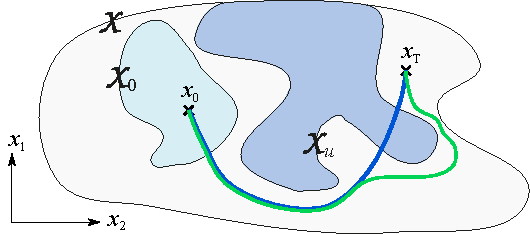
\includegraphics[width=0.75\textwidth]{safety.pdf}	
	\caption{Graphically interpretation of \autoref{eq:defsafety} in the state space. The blue trajectory is unsafe while the green trajectory is safe.}
	\label{fig:defsafety}
\end{figure}
\label{def_safety}
\end{exa}

\textbf{Beskriv forskellige m\aa der at h\aa ndtere constraint, samt beskriv deres fordele og ulemper!}

- \gls{mpc} \\
- \gls{clf} combined wiht \gls{cbf} (stabilization property of CLF
with the safety aspect from the CBF)   \\
- reference governor?\\

\gls{lie}

If the system always moves very slowly, acceleration may be ignored and maybe dyamics could be ignored altogether, only leaving the evolution of kinematics in the function $f(x)$.

The design of a safe controller features the property that a supplied control signal ensures compliance of the definition described in \autoref{sec:safety-def}.

A one-dimensional simple case is analysed at first. The approach adopted constitute the movement of instrument slide, see \autoref{fig:lol}.

\begin{figure}[H]
\center
--- NICE FIGURE OF INSTRUMENT SLIDE ---
\caption{nice figure}
\label{fig:lol}
\end{figure}

A barrier certificate function can be constructed from the definitions, i.e.:
\begin{flalign}
& B(x) \leq 0 \kk  \forall \hspace{0.3cm} x \in \mathcal{X}_0  \label{cer1}\\
& B(x) > 0  \kk  \forall \hspace{0.3cm} x \in \mathcal{X}_u \label{cer2} \\
& L_f(B(x)) \leq 0 \kk  \forall \hspace{0.3cm} x \in \mathcal{X} \label{cer3}
\end{flalign}
\vspace{-0.8cm}
\begin{longtable}{p{.9\textwidth} p{.1\textwidth} p{.1\textwidth}} 
Where  & & \\
\gls{bar} is the barrier function & [$\cdot$] \\ 
\end{longtable}
\vspace*{-0.2cm}
Based on \citep{bib:artstein}, which founded \gls{clf}s, a \gls{cbf} can be created \citep{bib:org_control}. With a system $\dot{x}=f(x)+g(x)u$, a \gls{cbf} exist if the below constraints are fulfilled:
\begin{flalign}
& x\in \mathcal{X}_u \hspace{0.3cm} \Rightarrow \hspace{0.3cm} B(x) > 0  \label{req1} \\
& L_gB(x) = 0 \hspace{0.3cm} \Rightarrow \hspace{0.3cm} L_fB(x) < 0 \label{req2} \\
& \{ x \in \mathcal{X} | B(x) \leq 0 \} \neq \emptyset \label{req3}
\end{flalign}
\vspace{-0.8cm}
\begin{longtable}{p{.9\textwidth} p{.1\textwidth} p{.1\textwidth}} 
Where  & & \\
$L_f(x)$ is the Lie derivative of $B(x)$ along the vector field  $f(x)$, i.e. $\frac{\partial B(x)}{\partial x}f(x)$ & [$\cdot$] \\ 
$L_f(x)$ is the Lie derivative of $B(x)$ along the vector field  $g(x)$, i.e. $\frac{\partial B(x)}{\partial x}g(x)$ & [$\cdot$] 
\end{longtable}
\vspace*{-0.2cm}
Taking a look at \autoref{req1} it states essentially the same as \autoref{cer2}, i.e. the unsafe area exist whenever $B(x)>0$. This makes it possible to design a unsafe region. \Autoref{req2} put forth the requirement that the gradient along the vector field $f(x)$ must point away from the barrier extremities whenever the input is with no significance (except for the critical point). \Autoref{req3} simply states that the safe area must contain some states as control otherwise is impossible.
\section{1-Dimensional Controller Design for Safety}
\subsubsection{Modelling of Slide Movement}
The slide movement is visualized in \autoref{fig:slidefig}.
\begin{figure}[H]
\center
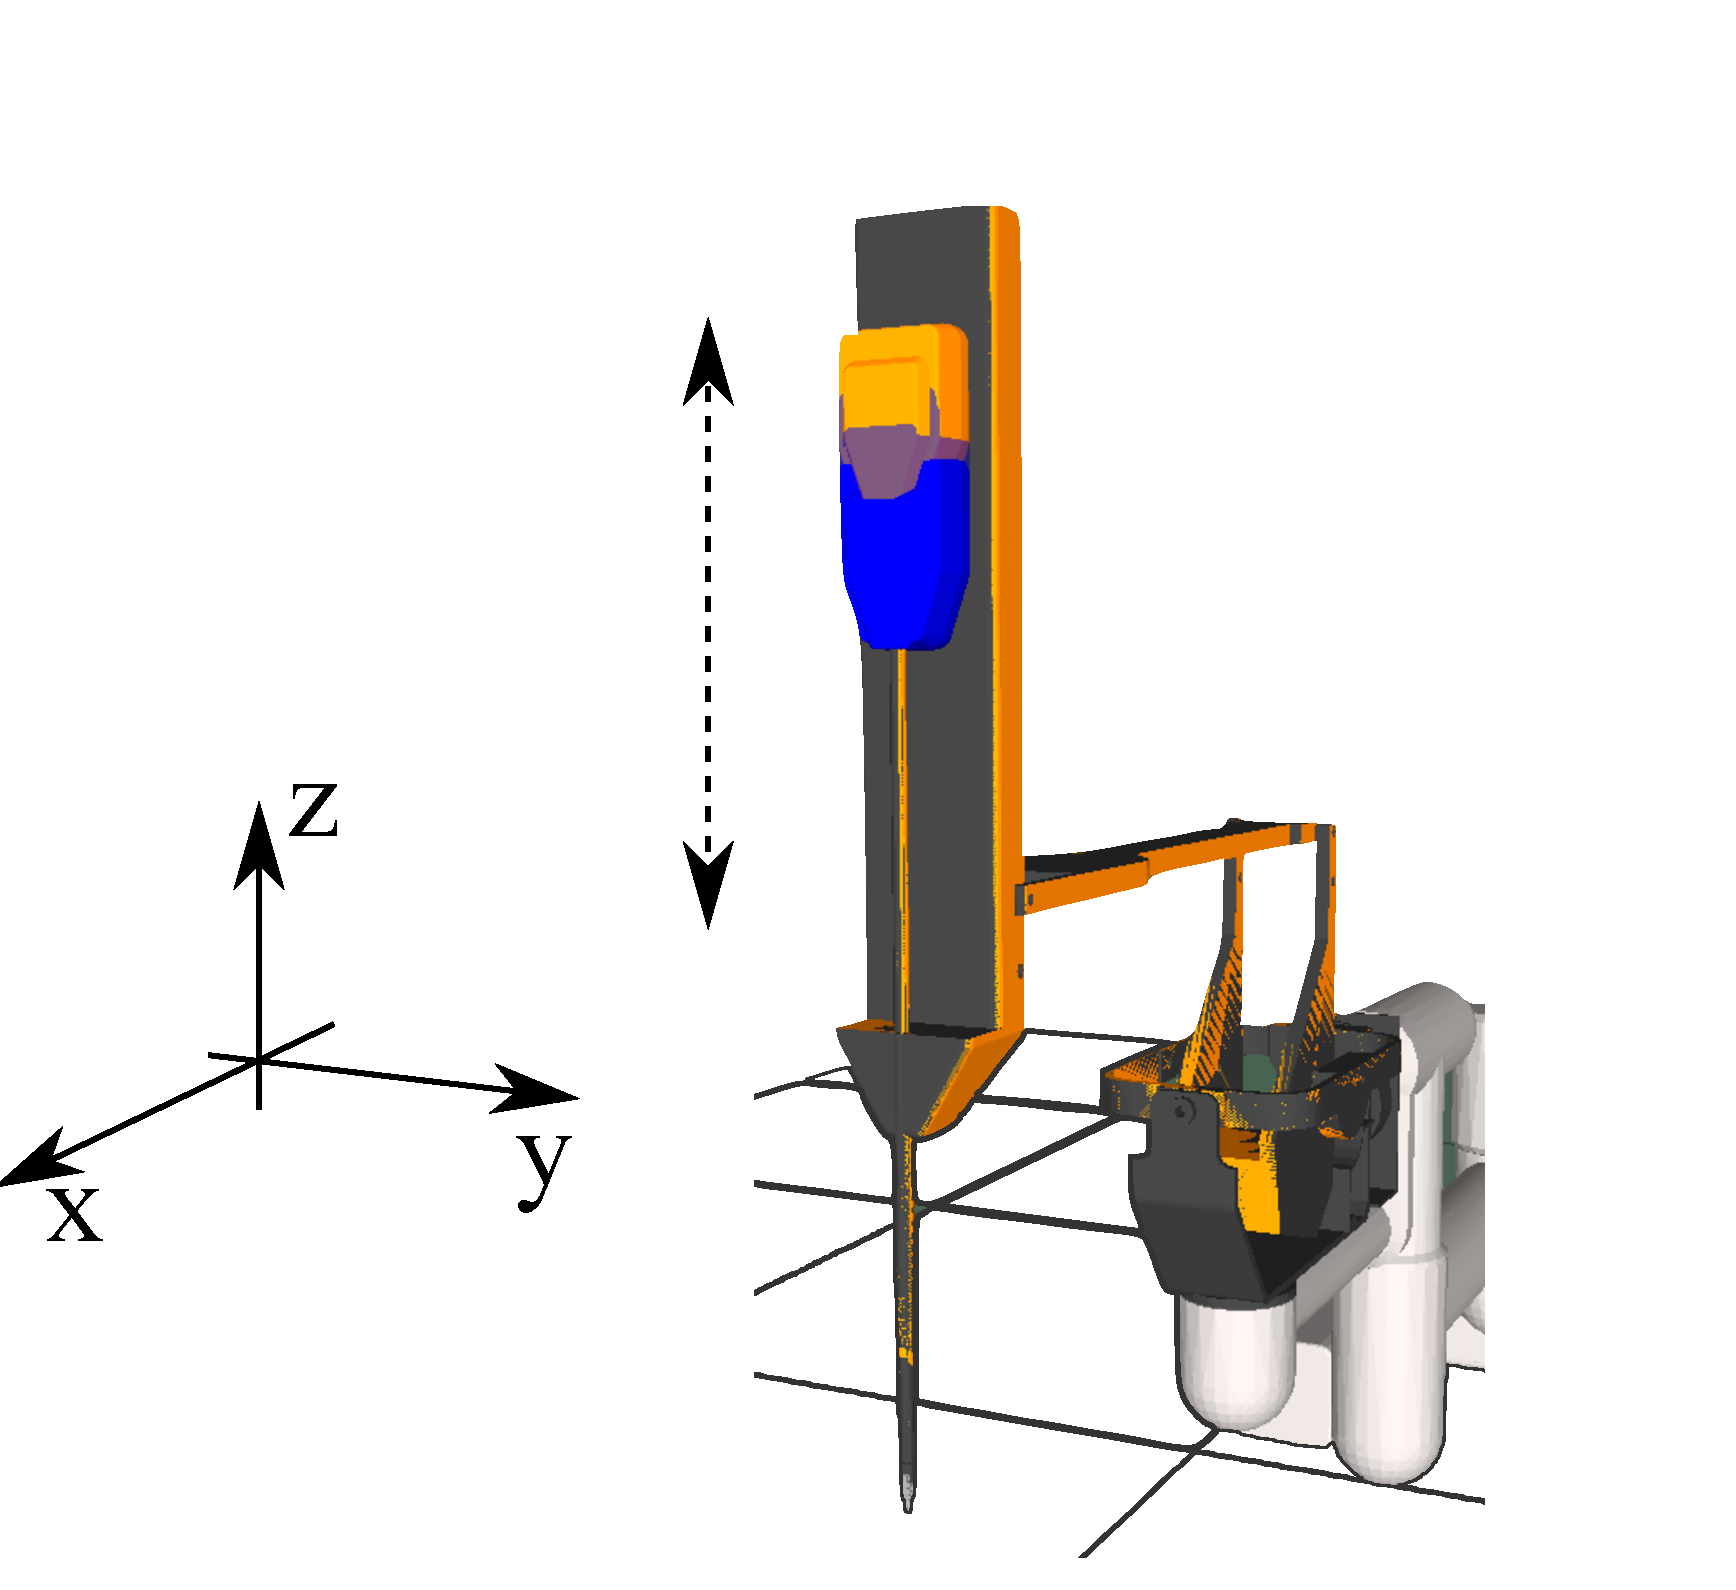
\includegraphics[scale=0.2]{slidemovefigure.pdf}
\caption{Slide movement which takes placed in the z-plane.}
\label{fig:slidefig}
\end{figure}

To obtain a model, a step response will be performed on the slide movement. The slide position can be measured by publishing the joint state angle in \gls{ros}. 

\hspace{1cm }\texttt{rostopic echo joint\_states/position[6]} \hspace{0.2cm} {\color{blue}{\# Be sure to have the ROS environment correctly configured according to \autoref{app:ros}}}

The step response is plotted in \autoref{fig:stepresponseslide}.
\begin{figure}[H]
\center
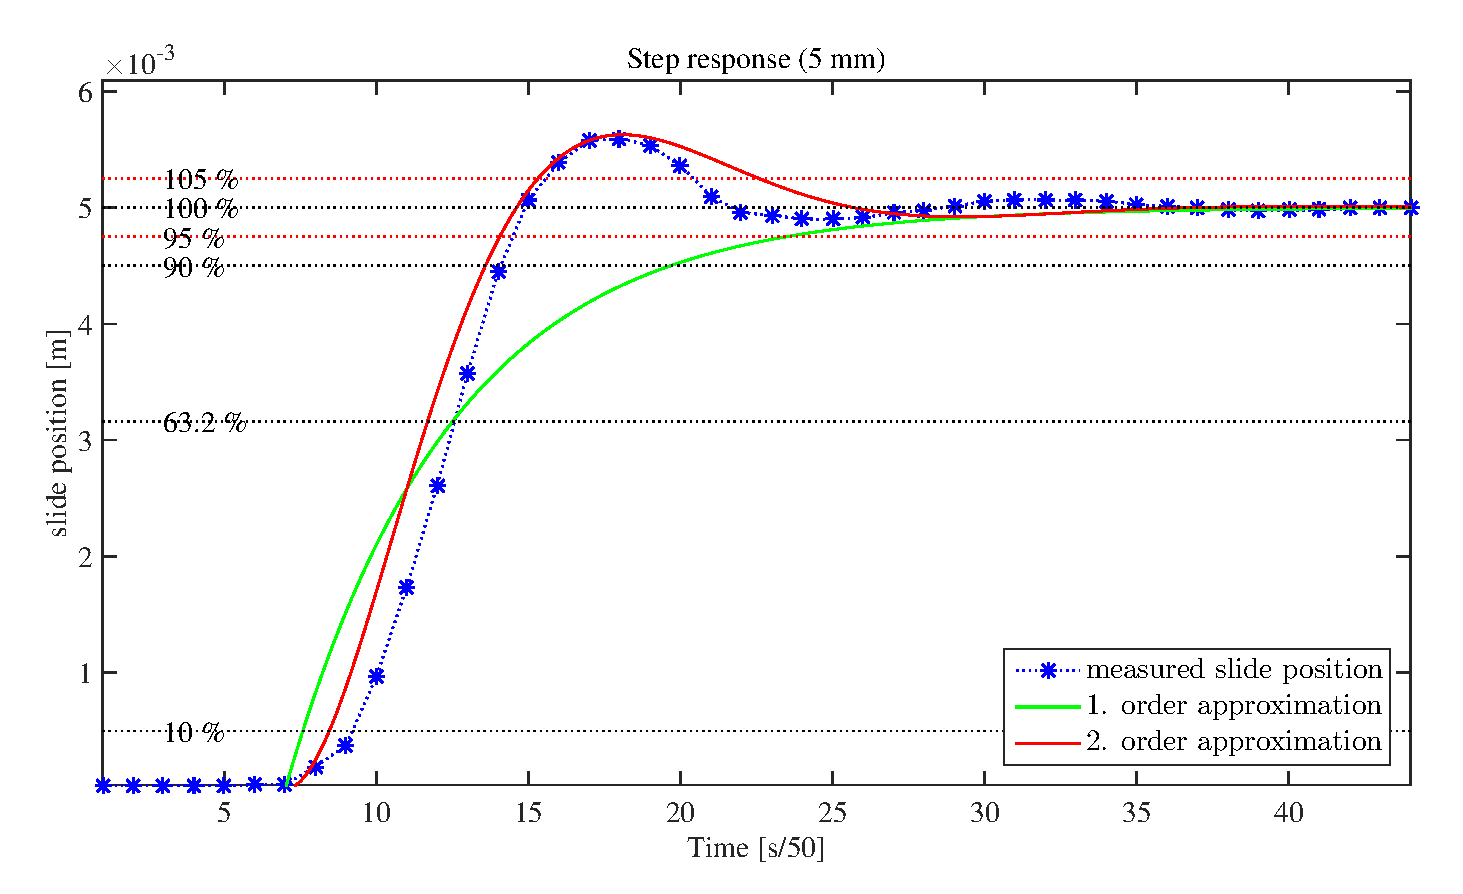
\includegraphics[scale=0.5]{step_slide.eps}
\caption{Step response from 0\,mm to 5\,mm. Plot details and measurements can be found in \autoref{app:cd} as \texttt{matlab\_scripts/slide\_step/plot\_slide\_pos.m}}
\label{fig:stepresponseslide}
\end{figure}

It is clear that this could be well approximated with an underdamped second order model (complex roots), however for initial simplicity and because modelling is not a focus point in this thesis, merely a simple model of the slide movement is used (it shall later be approximated to a second order model). It may, with some good will, be approximated to a linear first order system with a dominating time constant \gls{taus}: 
\begin{flalign*}
& Y(s) = \dfrac{1}{\tau_s s + 1}U(s) =  \dfrac{1/\tau_s}{s + 1/\tau_s}\,U(s) = (s+1/\tau_s)^{-1}\,1/\tau_s\,U(s) \kk  \overset{\overset{Y(s)=(C(sI-A)^{-1}B+D)U(s)}{\longrightarrow}}{\scriptsize \text{compare to obtain SS form}}  \\ 
& \dot{x} = \underbrace{-\tau_s^{-1}\,x}_{f_s(x)} + \underbrace{\tau_s^{-1}}_{g_s(x)} u
\end{flalign*}
Thus the system matrix $A$ and the input matrix $B$ can be seen easily. For the sake of generalization, they are named $f_s$ and $g_s$, i.e.:
\begin{flalign*}
f_s(x) = -\tau^{-1}x \kk \wedge \kk g_s(x) = \tau_s^{-1}
\end{flalign*}



The time constant $\tau_s$ can be measured by means of the matlab script found in ??? to:
\begin{flalign*}
\tau_s = 420\, \text{ms}
\end{flalign*} 
\subsubsection{Construction of Simple CBF}
To illustrate the usefulness of \gls{cbf}s, a palpable example hereof will be created with direct application to the Da Vinci robot. This example does not directly constitute application to a patient but favour the theory in a neat and comprehensible sense and secure a way to visual and physical verify the method.

A parabola is introduced as CBF. 
\begin{figure}[H]
\center
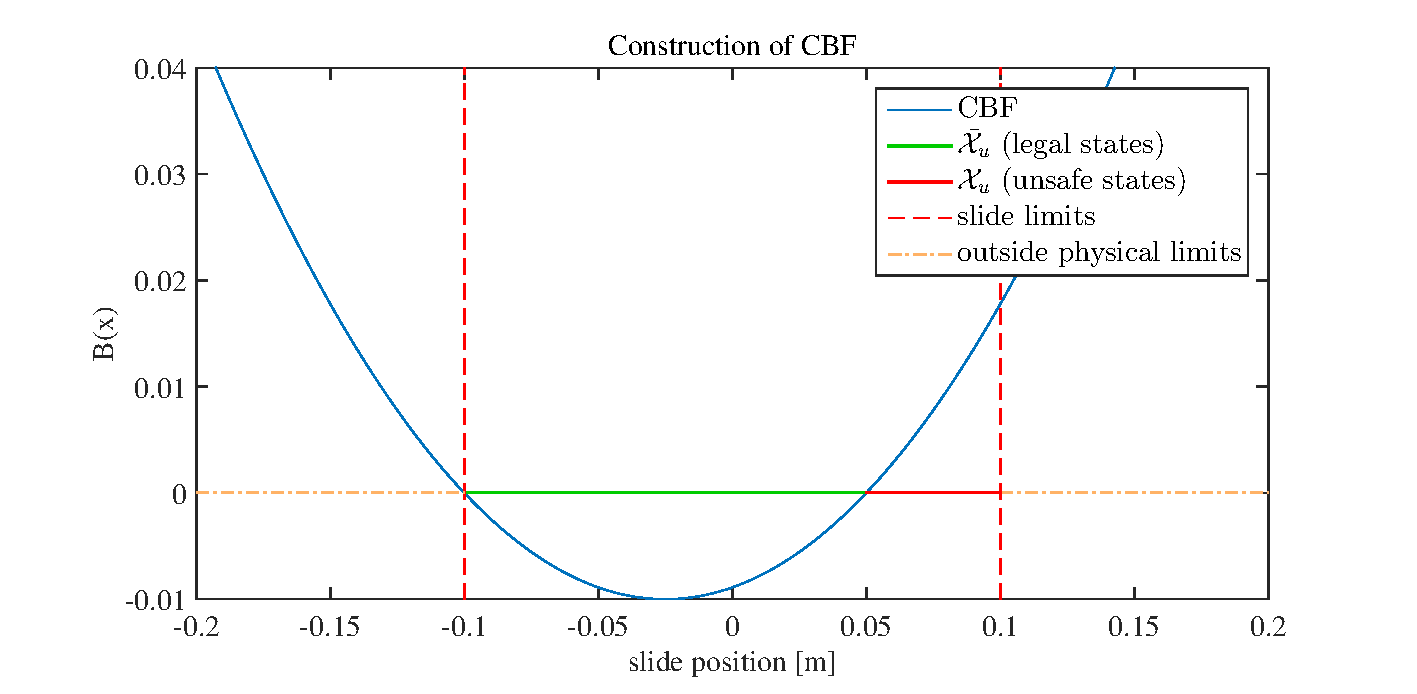
\includegraphics[scale=0.5]{parabel_1.eps}
\caption{nice figure}
\label{fig:lol}
\end{figure}